\documentclass[dvipdfmx]{jreport}
\usepackage{mypackage}
%%%%%%%%%%%%%%%%%%%%%%%%%%%%%%%%%%
\begin{document}

\chapter{統計}

\section{統計誤差}
磁場を光子のスピンと平行/反平行にかけた時のイベント数をそれぞれ$N_{+}$、$N_{-}$とすると大まかには$N_{+} \simeq N_{-}$なので、この二つの値が共に$N$程度であるとすると、アシンメトリー
\begin{equation}
  \label{asymmetry}
  \frac{N_{+} - N_{-}}{N_{+} + N_{-}}
\end{equation}
の統計誤差は誤差伝搬の式より$\frac{1}{\sqrt{N}}$となる。実験での期待されるアシンメトリー$\qty(\ref{asymmetry})$は約$0.08$なので、
統計誤差がその$10\%$になるのに必要なイベント数は$N_{+}$、$N_{-}$合わせて約$2*10^{4}$である。

\section{イベント数の見積}
\subsection{崩壊核子数の計算}
本実験では一回の照射で$100\mathrm{MBq}$の$\ce{Eu}$線源を作ることができる。このうち核異性体$\ce{^{152m}Eu}$の割合は?である。
放射能の初期値を
\begin{equation}
  A_0 = 100\mathrm{MBq}
\end{equation}
としたとき、強度は
\begin{equation}
  A\qty(t) = A_0 \cdot \exp(-\lambda \cdot t)
\end{equation}
で減衰する。ここで$\lambda$は崩壊定数と呼ばれ、半減期を$T=9.31\mathrm{h}$として
\begin{equation}
  \lambda = \frac{\ln(2)}{T}
\end{equation}
とかける。放射能$A\qty(t)$と核子数$N\qty(t)$との間には
\begin{equation}
  N\qty(t) = \frac{A\qty(t)}{\lambda}
\end{equation}
という関係があり、したがって照射後から時刻$t$までに崩壊する$\ce{^{152m}Eu}$の核子数$N_{\mathrm{decay}}$は
\begin{equation}
  N_{\mathrm{decay}} = N\qty(0) - N\qty(t) = \frac{A\qty(0) - A\qty(t)}{\lambda}
\end{equation}
と求まる。測定時間を$t=14\mathrm{h}$としたとき
\begin{equation}
  N_{\mathrm{decay}} = 3.58 \cdot 10^{12}
\end{equation}
となる。

\subsection{散乱体立体角の計算}
$6\mathrm{deg}$に対応する立体角は$0.03$、散乱体の角度を$10\mathrm{deg}$まで取ることにすると$10\mathrm{deg}$に対応する立体角は$0.09$なので、
散乱体方向の立体角の割合は$\frac{0.06}{4\pi}=0.004$となる。

\subsection{イベント数の見積}
一回の実験$\qty(14\mathrm{h})$で得られるイベント数は
\begin{equation}
  3.58 \cdot 10^{12} \times 0.13  \times e^{-\frac{5}{2.3}} \times 0.004 \times ^{-\frac{10}{9.8}} \times 0.5 \times 0.049
  \simeq 1.89 \times 10^{6} \mathrm{events}
\end{equation}
\begin{itemize}
\item $10^{12}$:本実験で測定時間の間に崩壊する$\ce{Eu}$核子数
\item $0.13$:$963\mathrm{keV}$の$\gamma$が放出される$\ce{^{152m}Eu}$のEC崩壊の分岐比
\item $e^{-\frac{5}{2.3}}$:鉄電磁石の中を$\gamma$が通過するときの減衰割合、$2.3\mathrm{cm}$は鉄中での$1\mathrm{MeV} \gamma$線の平均自由行程
\item $0.004$:$\ce{Eu}$線源から見た全立体角のうち、$\ce{Sm}$散乱体の方向の立体角の割合
\item $e^{-\frac{10}{9.8}}$:散乱体の中を$\gamma$が通過するときの減衰割合、$9.8\mathrm{cm}$は鉄中での$1\mathrm{MeV} \gamma$線の平均自由行程  
\item $0.5$:$\ce{Sm_{2}O_{3}}$共鳴散乱体から見た検出器方向への立体角の割合
\item $0.049$:$963\mathrm{keV} \gamma$線に対する$\ce{LaBr_{3}}$シンチレータの検出率
\end{itemize}

\section{バックグラウンドの考察}
本実験では$\ce{Sm_{2}O_{3}}$散乱体で散乱された後の$963\mathrm{keV}$と$841\mathrm{keV}$の$\gamma$を見たい。そこでこのエネルギー帯のバックグラウンドを考える。

\subsection{鉛シールドでのコンプトン散乱}
$974\mathrm{keV}$の$\gamma$が鉛シールドでコンプトン散乱され、$\ce{LaBr_{3}}$シンチレータに入ると$974\mathrm{keV}$を端とするコンプトンエッジが現れる。
この形は$\ce{LaBr_{3}}$シンチレータのエネルギー分解能に依存し、理想的には$974\mathrm{keV}$を端とするステップ関数になるが、
実際にADCで見ることのできるスペクトラムは、図$\ref{spectrum}$にあるようなガウシアンとの畳み込みが観測される。
\begin{figure}[htbp]
  \centering
  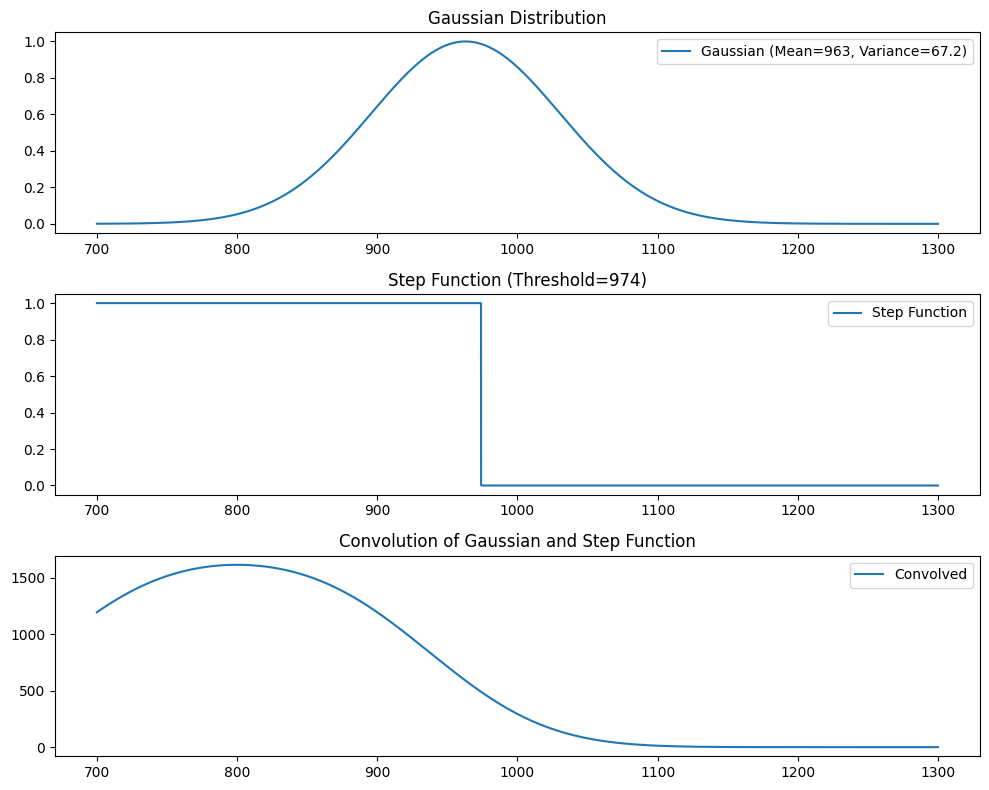
\includegraphics[width=100mm]{figure/spectrum.png}
  \caption{スペクトル \label{spectrum}}
\end{figure}

\subsection{環境放射線}
そのほかに考えられるノイズとしては環境放射線が挙げられる。特に今回観測したいエネルギー帯に寄与するものとしては、図$\ref{ウラン}$と図$\ref{トリウム}$に示すようなウラン系列とトリウム系列がある。
\begin{itemize}
\item $\ce{^{228}Ac}$ $836\mathrm{keV}$ $\qty(トリウム系列)$
\item $\ce{^{208}Tl}$ $861\mathrm{keV}$ $\qty(トリウム系列)$
\item $\ce{^{228}Ac}$ $911\mathrm{keV}$ $\qty(トリウム系列)$
\item $\ce{^{214}Bi}$ $934\mathrm{keV}$ $\qty(ウラン系列)$
\item $\ce{^{228}Ac}$ $965\mathrm{keV}$ $\qty(トリウム系列)$
\item $\ce{^{228}Ac}$ $969\mathrm{keV}$ $\qty(トリウム系列)$
\end{itemize}
\begin{figure}[htbp]
  \centering
  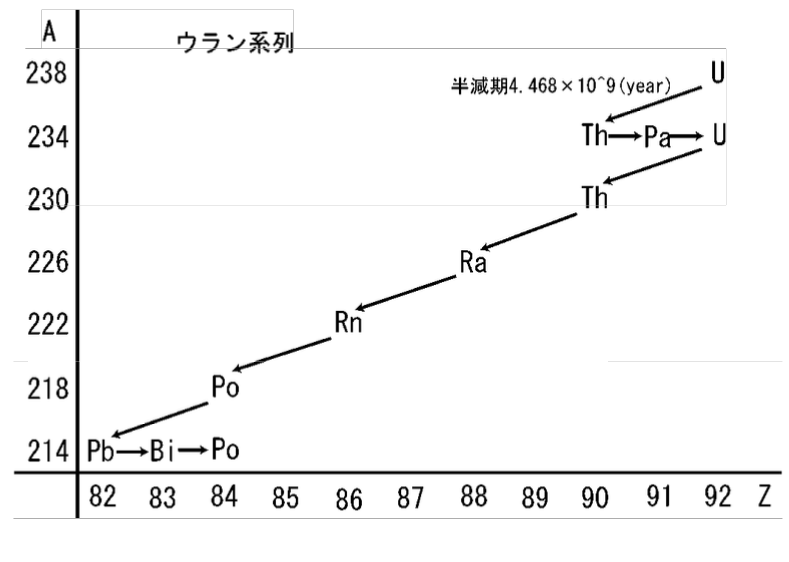
\includegraphics[width=100mm]{figure/uran.png}
  \caption{ウラン系列 \label{ウラン}}
\end{figure}
\begin{figure}[htbp]
  \centering
  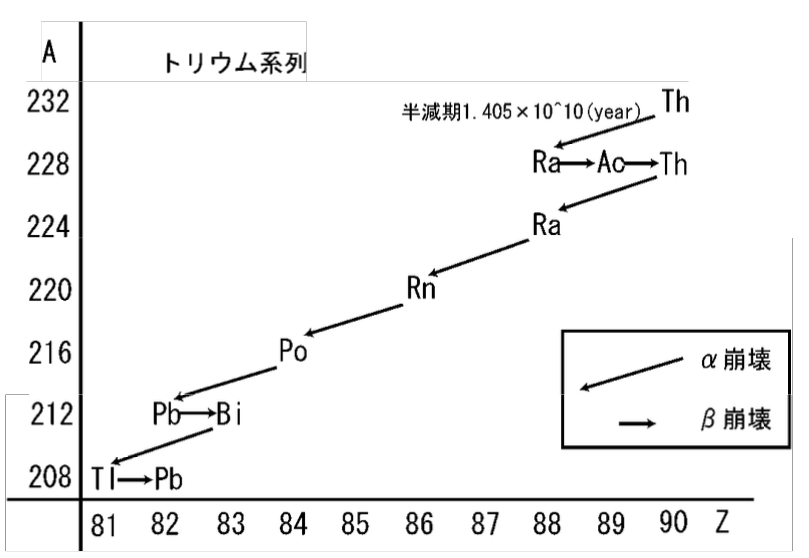
\includegraphics[width=100mm]{figure/trium.png}
  \caption{トリウム系列 \label{トリウム}}
\end{figure}

\subsection{環境放射線の測定}
\begin{figure}[htbp]
  \centering
  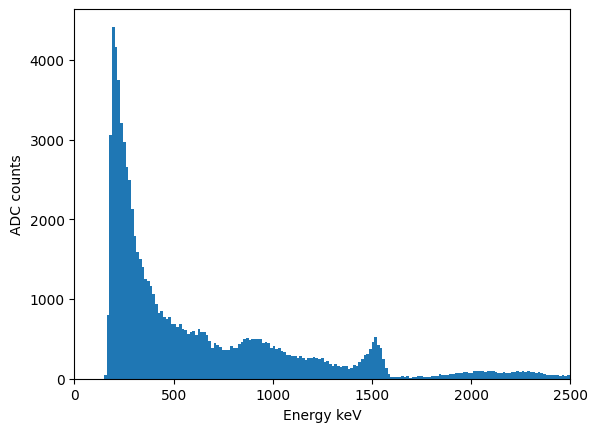
\includegraphics[width=100mm]{figure/background.png}
  \caption{遮蔽なしのバックグラウンド \label{background}}
\end{figure}
\begin{figure}[htbp]
  \centering
  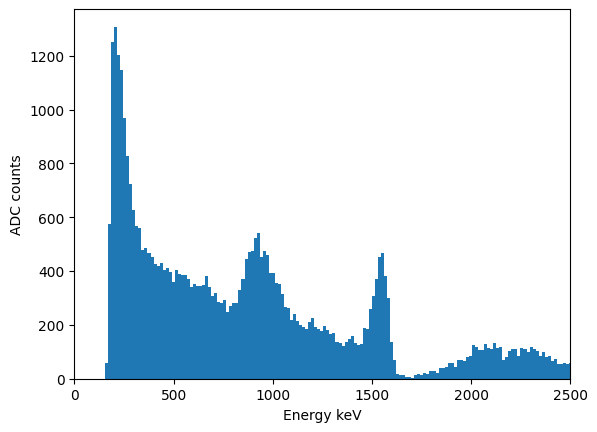
\includegraphics[width=100mm]{figure/background_attenated.png}
  \caption{遮蔽ありのバックグラウンド \label{background_attenated}}
\end{figure}

\end{document}
